\documentclass{article}

% Language setting
% Replace `english' with e.g. `spanish' to change the document language
\usepackage[italian]{babel}

% Set page size and margins
% Replace `letterpaper' with `a4paper' for UK/EU standard size
\usepackage[a4paper,top=2cm,bottom=2cm,left=2.5cm,right=2.5cm,marginparwidth=1.75cm]{geometry}

% Useful packages
\usepackage{amsmath}
\usepackage{graphicx}
\usepackage[colorlinks=true, allcolors=blue]{hyperref}
\usepackage{caption}
\usepackage{subcaption}
\usepackage{listings} % For code blocks
\usepackage[parfill]{parskip} % For avoiding auto indent every new line

\graphicspath{ {./images/} }

\title{Documentazione di progetto\\ Business Intelligence per i Servizi Finanziari}
\author{Tommaso Cammelli, 851593}

\begin{document}
\maketitle

\section{Sommario dei dati utilizzati}

\subsection{Presentazione e descrizione dei titoli selezionati}

Per questo progetto sono stati presi in considerazione 6 titoli azionari, appartenenti a 3 settori diversi:

\begin{itemize}
    \item \textbf{Settore tecnologico}: Meta Platforms, Inc. (FB), Alphabet Inc. (GOOG)
    \item \textbf{Settore militare}: Raytheon Technologies Corporation (RTX),\\ Lockheed Martin Corporation (LMT)
    \item \textbf{Settore bancario}: Bank of America Corporation (BAC), JPMorgan Chase \& Co. (JPM)
\end{itemize}

\textbf{Motivazione per scelta dei titoli}

\begin{itemize}
  \item \textbf{Meta Platforms, Inc. (FB)}: Ho scelto questo titolo in quanto è una delle aziende con la \emph{market capitalization} più alta nel mondo\footnote{pagina web di referenza: \href{https://companiesmarketcap.com/tech/largest-tech-companies-by-market-cap/}{https://companiesmarketcap.com/tech/largest-tech-companies-by-market-cap/}},
  e facendo parte del \emph{faang}\footnote{Acronimo dei cinque top stocks americani nel settore tecnologico, \href{https://www.investopedia.com/terms/f/faang-stocks.asp}{https://www.investopedia.com/terms/f/faang-stocks.asp}} ho ritenuto interessante
  valutare il comportamento di questo titolo durante eventi controversi.

  \item \textbf{Alphabet Inc. (GOOG)}: todo
  
  \item \textbf{Raytheon Technologies Corporation (RTX)}: todo
  
  \item \textbf{Lockheed Martin Corporation (LMT)}: todo
  
  \item \textbf{Bank of America Corporation (BAC)}: todo
  
  \item \textbf{JPMorgan Chase \& Co. (JPM)}: todo
\end{itemize}

\subsection{Funzioni utilizzate per download e fusione}

Per il download dei dati da Yahoo! Finance\footnote{\href{https://finance.yahoo.com}{https://finance.yahoo.com}} è stata utilizzata la nota libreria di python
yfinance\footnote{Libreria FOSS per download di dati finanziari da Yahoo! finance, \href{https://pypi.org/project/yfinance/}{https://pypi.org/project/yfinance/}} dove attraverso la funzione
\emph{download()} ha permesso di scaricare i dati di interesse nel periodo rilevante per questo progetto.

\begin{lstlisting}[language=Python]
  # Esempio di download da Yahoo! Finance dello storico prezzi di FB
  import yfinance as yf

  fb_df = yf.download('FB', start='2011-11-30', end='2021-11-30')
\end{lstlisting}

Relativamente alla fusione dei dati scaricati in un unico DataFrame di Pandas\footnote{Libreria per data analysis e manipulation, 
\href{https://pandas.pydata.org/}{https://pandas.pydata.org/}} è stata utilizzata la funzione \emph{DataFrame()} 
per creare un nuovo dataframe vuoto, sono stati poi usati i costrutti base di python per popolare il dataframe con i nostri dati di interesse.

\begin{lstlisting}[language=Python]
  # Esempio di fusione dei dati da due indici scaricati precedentemente
  import pandas as pd

  adj_close_tot = pd.DataFrame()
  adj_close_tot["Meta Price"] = fb_df[["Adj Close"]]
  adj_close_tot["Alphabet Price"] = goog_df[["Adj Close"]]
\end{lstlisting}

\pagebreak

\subsection{presentazione dei dati}

Rappresentiamo i dati ottenuti tramite un grafico a linee che si trova alla figura \ref{fig:all_stocks_price} dove 
si mostra la variazione di prezzo di tutti gli stock considerati in questo progetto\footnote{FB, GOOG, RTX, LMT, BAC, JPM} nel periodo 
da 30-11-2011 a 30-11-2021.

\begin{figure}[h]
  \centering
  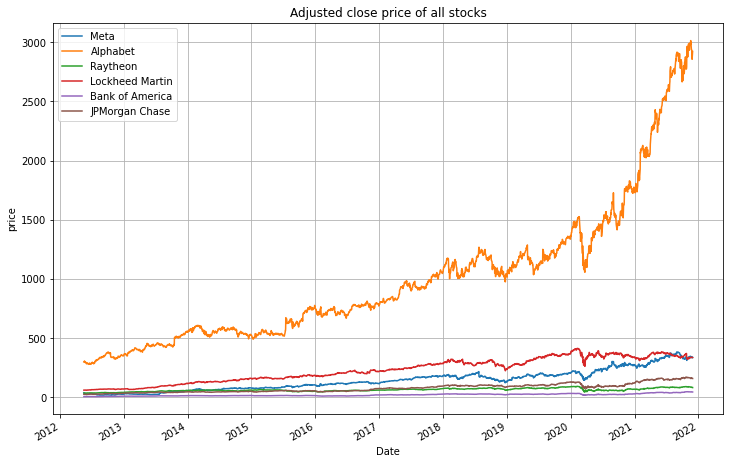
\includegraphics[width=0.7\textwidth]{all_stocks_price.png}
  \caption{grafico con prezzo degli stock da 18/05/2012 a 30/11/2021}
  \label{fig:all_stocks_price}
\end{figure}

Tutti i grafici del progetto sono stati generati utilizzando la libreria di python \emph{matplotlib}\footnote{Libreria per creare visualizzazioni dei dati anche interattive in Python, \href{https://matplotlib.org}{https://matplotlib.org}}
che tramite apposite funzioni ha permesso la quasi totale personalizzazione dei grafici per semplificare la lettura dei dati.

Rappresentiamo ora alla figura \ref{fig:all_stocks_table_10} le prime 10 righe della tabella che contiene il prezzo combinato di tutti gli stock considerati (stessa tabella utilizzata per il plot del grafico qui sopra), 
fusi in un solo \emph{DataFrame} grazie a \emph{Pandas}.

\begin{figure}[h]
  \centering
  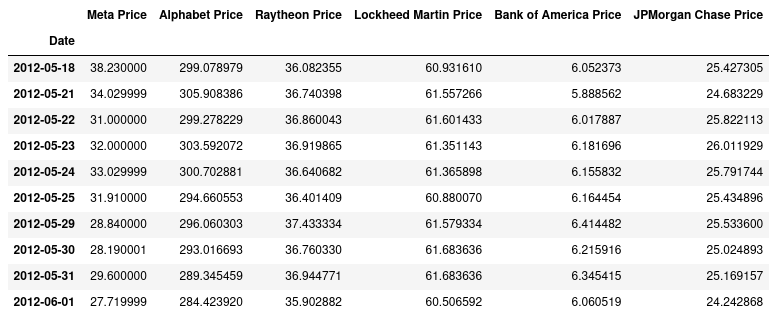
\includegraphics[width=0.7\textwidth]{stocks_combined_first_10.png}
  \caption{tabella con prezzo degli stock da 18/05/2012 a 30/11/2021 (prime 10 righe)}
  \label{fig:all_stocks_table_10}
\end{figure}

\textbf{Nota:} Meta Platforms, Inc. (FB) è stata quotata in borsa solo a partire dal 18/05/2012, a causa di ciò i dati aggregati partono
solo da quella data.

\section{Statistiche descrittive}

\subsection{Settore tecnologico}

Statistiche descrittive dei due titoli relativi al settore tecnologico FB e GOOG.

\subsubsection{Rendimenti semplici e composti}

osserva i due grafici \ref{fig:rendimenti_semplici_tecno} e \ref{fig:rendimenti_compositi_tecno}, sono importanti

\begin{figure}[h]
    \centering
    \begin{minipage}{.5\textwidth}
      \centering
      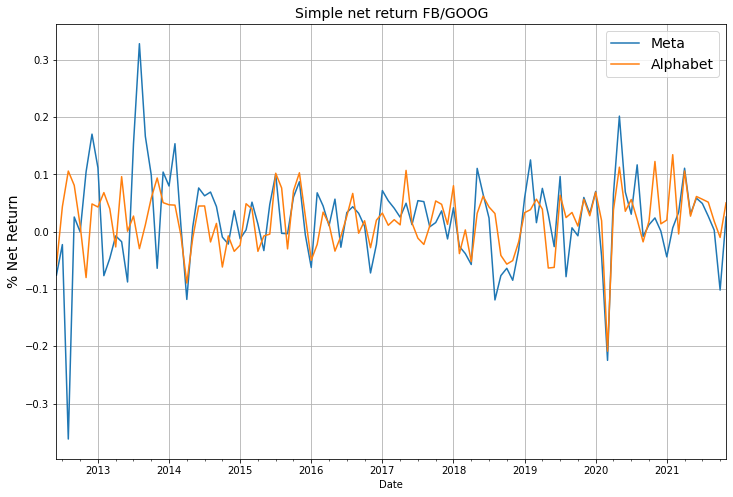
\includegraphics[width=1\linewidth]{tecno_rendimenti_semplici_netti.png}
      \captionof{figure}{Rendimenti semplici netti FB e GOOG}
      \label{fig:rendimenti_semplici_tecno}
    \end{minipage}%
    \begin{minipage}{.5\textwidth}
      \centering
      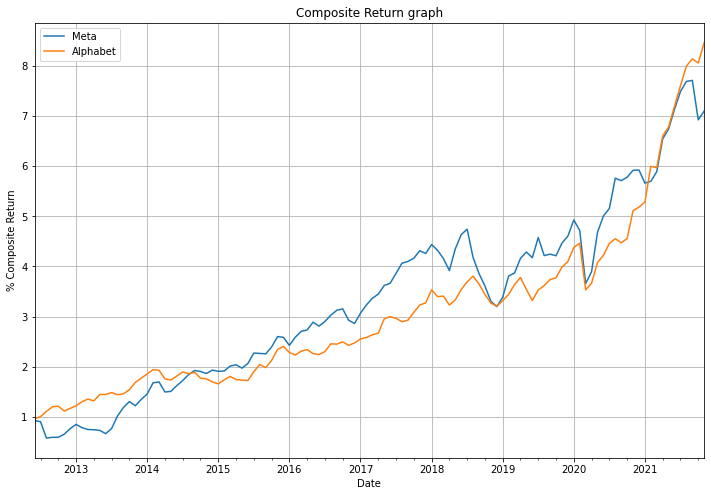
\includegraphics[width=.97\linewidth]{tecno_rendimenti_composti.png}
      \captionof{figure}{Rendimenti compositi FB e GOOG}
      \label{fig:rendimenti_compositi_tecno}
    \end{minipage}
    \end{figure}


\subsection{How to include Figures}

Note that your figure will automatically be placed in the most appropriate place for it, given the surrounding text and taking into account other figures or tables that may be close by. You can find out more about adding images to your documents in this help article on \href{https://www.overleaf.com/learn/how-to/Including_images_on_Overleaf}{including images on Overleaf}.


\subsection{How to add Tables}

Use the table and tabular environments for basic tables --- see Table~\ref{tab:widgets}, for example. For more information, please see this help article on \href{https://www.overleaf.com/learn/latex/tables}{tables}. 

\begin{table}
\centering
\begin{tabular}{l|r}
Item & Quantity \\\hline
Widgets & 42 \\
Gadgets & 13
\end{tabular}
\caption{\label{tab:widgets}An example table.}
\end{table}

\subsection{How to add Comments and Track Changes}

Comments can be added to your project by highlighting some text and clicking ``Add comment'' in the top right of the editor pane. To view existing comments, click on the Review menu in the toolbar above. To reply to a comment, click on the Reply button in the lower right corner of the comment. You can close the Review pane by clicking its name on the toolbar when you're done reviewing for the time being.

Track changes are available on all our \href{https://www.overleaf.com/user/subscription/plans}{premium plans}, and can be toggled on or off using the option at the top of the Review pane. Track changes allow you to keep track of every change made to the document, along with the person making the change. 

\subsection{How to add Lists}

You can make lists with automatic numbering \dots

\begin{enumerate}
\item Like this,
\item and like this.
\end{enumerate}
\dots or bullet points \dots
\begin{itemize}
\item Like this,
\item and like this.
\end{itemize}

\subsection{How to write Mathematics}

\LaTeX{} is great at typesetting mathematics. Let $X_1, X_2, \ldots, X_n$ be a sequence of independent and identically distributed random variables with $\text{E}[X_i] = \mu$ and $\text{Var}[X_i] = \sigma^2 < \infty$, and let
\[S_n = \frac{X_1 + X_2 + \cdots + X_n}{n}
      = \frac{1}{n}\sum_{i}^{n} X_i\]
denote their mean. Then as $n$ approaches infinity, the random variables $\sqrt{n}(S_n - \mu)$ converge in distribution to a normal $\mathcal{N}(0, \sigma^2)$.


\subsection{How to change the margins and paper size}

Usually the template you're using will have the page margins and paper size set correctly for that use-case. For example, if you're using a journal article template provided by the journal publisher, that template will be formatted according to their requirements. In these cases, it's best not to alter the margins directly.

If however you're using a more general template, such as this one, and would like to alter the margins, a common way to do so is via the geometry package. You can find the geometry package loaded in the preamble at the top of this example file, and if you'd like to learn more about how to adjust the settings, please visit this help article on \href{https://www.overleaf.com/learn/latex/page_size_and_margins}{page size and margins}.

\subsection{How to change the document language and spell check settings}

Overleaf supports many different languages, including multiple different languages within one document. 

To configure the document language, simply edit the option provided to the babel package in the preamble at the top of this example project. To learn more about the different options, please visit this help article on \href{https://www.overleaf.com/learn/latex/International_language_support}{international language support}.

To change the spell check language, simply open the Overleaf menu at the top left of the editor window, scroll down to the spell check setting, and adjust accordingly.

\subsection{How to add Citations and a References List}

You can simply upload a \verb|.bib| file containing your BibTeX entries, created with a tool such as JabRef. You can then cite entries from it, like this: \cite{greenwade93}. Just remember to specify a bibliography style, as well as the filename of the \verb|.bib|. You can find a \href{https://www.overleaf.com/help/97-how-to-include-a-bibliography-using-bibtex}{video tutorial here} to learn more about BibTeX.

If you have an \href{https://www.overleaf.com/user/subscription/plans}{upgraded account}, you can also import your Mendeley or Zotero library directly as a \verb|.bib| file, via the upload menu in the file-tree.

\subsection{Good luck!}

We hope you find Overleaf useful, and do take a look at our \href{https://www.overleaf.com/learn}{help library} for more tutorials and user guides! Please also let us know if you have any feedback using the Contact Us link at the bottom of the Overleaf menu --- or use the contact form at \url{https://www.overleaf.com/contact}.

\bibliographystyle{alpha}
\bibliography{sample}

\end{document}